
%(BEGIN_QUESTION)
% Copyright 2010, Tony R. Kuphaldt, released under the Creative Commons Attribution License (v 1.0)
% This means you may do almost anything with this work of mine, so long as you give me proper credit

A brand-new control system for a chemical reaction process uses a variable-frequency drive (VFD) to control the speed of the charge pump introducing chemical fluids into a reaction vessel.  This VFD gets a 4-20 mA control signal from one of the channels of an analog output card on a programmable logic controller (PLC).  The PLC in turn receives operating instructions from a touch-screen panel (``HMI'') where the operators can monitor and control the process:

$$\includegraphics[width=15.5cm]{i00067x01.eps}$$

This system is newly constructed, and has not yet worked.  The operators try starting up the pump by pressing the ``Pump start'' icon on the touch-screen, but nothing happens.  A technician disconnects the signal cable from the PLC's analog output terminals and then connects the cable's end to a ``loop calibrator'' to send 12 mA DC to the VFD for a test.  At this, the motor starts up and runs at half speed.  

Identify the likelihood of each specified fault for this circuit.  Consider each fault one at a time (i.e. no coincidental faults), determining whether or not each fault could independently account for {\it all} measurements and symptoms in this circuit.

% No blank lines allowed between lines of an \halign structure!
% I use comments (%) instead, so that TeX doesn't choke.

$$\vbox{\offinterlineskip
\halign{\strut
\vrule \quad\hfil # \ \hfil & 
\vrule \quad\hfil # \ \hfil & 
\vrule \quad\hfil # \ \hfil \vrule \cr
\noalign{\hrule}
%
% First row
{\bf Fault} & {\bf Possible} & {\bf Impossible} \cr
%
\noalign{\hrule}
%
% Another row
Circuit breaker off &  & \cr
%
\noalign{\hrule}
%
% Another row
Touch-screen panel malfunctioning &  & \cr
%
\noalign{\hrule}
%
% Another row
Programming error in PLC &  & \cr
%
\noalign{\hrule}
%
% Another row
Faulted power cable between VFD and motor &  & \cr
%
\noalign{\hrule}
%
% Another row
Faulted power cable between breaker and VFD &  & \cr
%
\noalign{\hrule}
%
% Another row
Analog output card malfunctioning &  & \cr
%
\noalign{\hrule}
%
% Another row
Shorted signal cable &  & \cr
%
\noalign{\hrule}
} % End of \halign 
}$$ % End of \vbox

Finally, identify the {\it next} diagnostic test or measurement you would make on this system.  Explain how the result(s) of this next test or measurement help further identify the location and/or nature of the fault.

\vfil

\underbar{file i00067}
\eject
%(END_QUESTION)





%(BEGIN_ANSWER)

This is a graded question -- no answers or hints given!

%(END_ANSWER)





%(BEGIN_NOTES)

A useful diagnostic strategy is to map the flow of data and of power between components in the system, in order to clearly establish the cause-and-effect relationships between them.  Blue arrows show the direction of {\it data} flow in the system, while red arrows show the direction of {\it power} flow in the system.  Any fault in a component will, of course, affect the operation of components ``downstream'' of the failed component:

$$\includegraphics[width=15.5cm]{i00067x02.eps}$$

We are told the motor runs when a 12 mA signal is injected into the analog signal cable using a loop calibrator.  This tells us the motor, VFD, and circuit breaker must all be functioning properly.  If the motor is not running as commanded from the HMI, it means the problem must lie in the PLC, the HMI, or the cable connecting those two components together.

% No blank lines allowed between lines of an \halign structure!
% I use comments (%) instead, so that TeX doesn't choke.

$$\vbox{\offinterlineskip
\halign{\strut
\vrule \quad\hfil # \ \hfil & 
\vrule \quad\hfil # \ \hfil & 
\vrule \quad\hfil # \ \hfil \vrule \cr
\noalign{\hrule}
%
% First row
{\bf Fault} & {\bf Possible} & {\bf Impossible} \cr
%
\noalign{\hrule}
%
% Another row
Circuit breaker off &  & $\surd$ \cr
%
\noalign{\hrule}
%
% Another row
Touch-screen panel malfunctioning & $\surd$  & \cr
%
\noalign{\hrule}
%
% Another row
Programming error in PLC & $\surd$  & \cr
%
\noalign{\hrule}
%
% Another row
Faulted power cable between VFD and motor &  & $\surd$ \cr
%
\noalign{\hrule}
%
% Another row
Faulted power cable between breaker and VFD &  & $\surd$ \cr
%
\noalign{\hrule}
%
% Another row
Analog output card malfunctioning & $\surd$  & \cr
%
\noalign{\hrule}
%
% Another row
Shorted signal cable &  & $\surd$ \cr
%
\noalign{\hrule}
} % End of \halign 
}$$ % End of \vbox

One possible diagnostic test would be to use a laptop PC to connect to the PLC and check the analog output register value.  The idea here would be to determine whether or not the PLC program is even trying to generate a signal to tell the VFD to run.  If the output register shows a significant value (i.e. a value large enough that the VFD should be running), it means the analog output channel is likely defective.  If the output register shows zero (or some other insignificant value), it means the program is not writing the necessary number to that register, and it is likely a programming problem.

A test not requiring a laptop PC would be to measure the current being sent from the card to the VFD.  If this current is below 4 mA, the problem is likely a hardware fault in the analog output card.  If the current is 4 mA, the problem is likely programming-related.

%INDEX% Basics, control loop troubleshooting: determining reason why VFD won't run
%INDEX% Final Control Elements: troubleshooting
%INDEX% PLC, troubleshooting: motor start/stop control circuit

%(END_NOTES)


